\subsubsection{Module MD-02: Quản lý Thực đơn \& Sản phẩm}
\begin{longtable}{|m{2cm}|m{2.5cm}|m{2cm}|m{4cm}|m{4.5cm}|}
\caption{Danh sách Yêu cầu Chức năng cho Module MD-02: Quản lý Thực đơn \& Sản phẩm} \label{tab:fr_md02} \\
\hline
\textbf{Mã Module} & \textbf{Mã Yêu cầu CN} & \textbf{Mã Người dùng} & \textbf{Tên Chức năng} & \textbf{Mô tả Ngắn} \\
\hline
\endhead % Header cho các trang tiếp theo

\hline
\endfoot % Footer cho bảng

\hline
\endlastfoot % Footer cho trang cuối cùng

MD-02 & FR-MD02-01 & US-01 & Tạo Sản phẩm Mới (Món ăn/Đồ uống) & Cho phép Quản lý nhà hàng thêm một món ăn, đồ uống, hoặc dịch vụ mới vào hệ thống với các thông tin cơ bản (tên, giá, loại). \\
\hline
MD-02 & FR-MD02-02 & US-01 & Chỉnh sửa Thông tin Sản phẩm & Cho phép Quản lý nhà hàng cập nhật các chi tiết của một sản phẩm đã tồn tại (ví dụ: thay đổi giá bán, mô tả, cập nhật hình ảnh, gán lại danh mục). \\
\hline
MD-02 & FR-MD02-03 & US-01 & Lưu trữ/Hủy kích hoạt Sản phẩm & Cho phép Quản lý nhà hàng ẩn một sản phẩm khỏi các giao dịch (ví dụ: POS, đặt hàng online) mà không xóa hẳn dữ liệu lịch sử. \\
\hline
MD-02 & FR-MD02-04 & US-01 & Quản lý Danh mục Sản phẩm POS & Cho phép Quản lý nhà hàng tạo, sửa, xóa và sắp xếp thứ tự các danh mục được sử dụng để nhóm sản phẩm trên giao diện POS (ví dụ: Khai vị, Món chính, Tráng miệng, Đồ uống). \\
\hline
MD-02 & FR-MD02-05 & US-01 / US-10 & Định nghĩa Thuộc tính \& Giá trị (cho Biến thể) & Cho phép người dùng định nghĩa các thuộc tính (ví dụ: Kích cỡ, Độ cay, Loại topping) và các giá trị tương ứng cho từng thuộc tính (ví dụ: S, M, L; Ít cay, Cay vừa, Cay nhiều; Phô mai, Thịt nguội). \\
\hline
MD-02 & FR-MD02-06 & US-01 & Cấu hình Biến thể Sản phẩm & Cho phép Quản lý nhà hàng áp dụng các thuộc tính đã định nghĩa vào một sản phẩm gốc để tạo ra các biến thể (ví dụ: Cà phê size S, Cà phê size L), quản lý giá và mã SKU riêng cho từng biến thể nếu cần. \\
\hline
MD-02 & FR-MD02-07 & US-01 & Thiết lập Loại Sản phẩm & Cho phép Quản lý nhà hàng xác định loại sản phẩm (Consumable, Stockable, Service) để quyết định cách hệ thống quản lý tồn kho (nếu là Stockable) hoặc không theo dõi tồn kho. \\
\hline
MD-02 & FR-MD02-08 & US-01 & Cấu hình Hiển thị trên POS & Cho phép Quản lý nhà hàng đánh dấu sản phẩm có sẵn sàng để bán trên POS hay không và gán sản phẩm vào (các) danh mục POS phù hợp. \\
\hline
MD-02 & FR-MD02-09 & US-01 & Quản lý Hình ảnh Sản phẩm & Cho phép Quản lý nhà hàng tải lên và quản lý hình ảnh đại diện cho sản phẩm, hiển thị trên POS hoặc các kênh bán hàng khác. \\
\hline
MD-02 & FR-MD02-10 & US-01 & Cấu hình In Bếp/Hiển thị KDS & Cho phép Quản lý nhà hàng chỉ định danh mục sản phẩm nào sẽ được gửi đến máy in bếp hoặc màn hình KDS cụ thể khi đặt hàng qua POS. (Có thể liên quan cấu hình POS/IoT). \\
\hline
MD-02 & FR-MD02-11 & US-01 & Định nghĩa Sản phẩm Tùy chọn/Phụ thu & Cho phép Quản lý nhà hàng tạo các sản phẩm nhỏ (ví dụ: Extra cheese, Thêm sốt) để dùng làm tùy chọn có tính phí khi khách hàng yêu cầu thêm vào món chính (sử dụng trong cấu hình POS modifiers). \\
\hline

\end{longtable}

\subsubsubsection{FR-MD01-01: Tạo ca làm việc mới}

\begin{figure}[H]
	\centering
	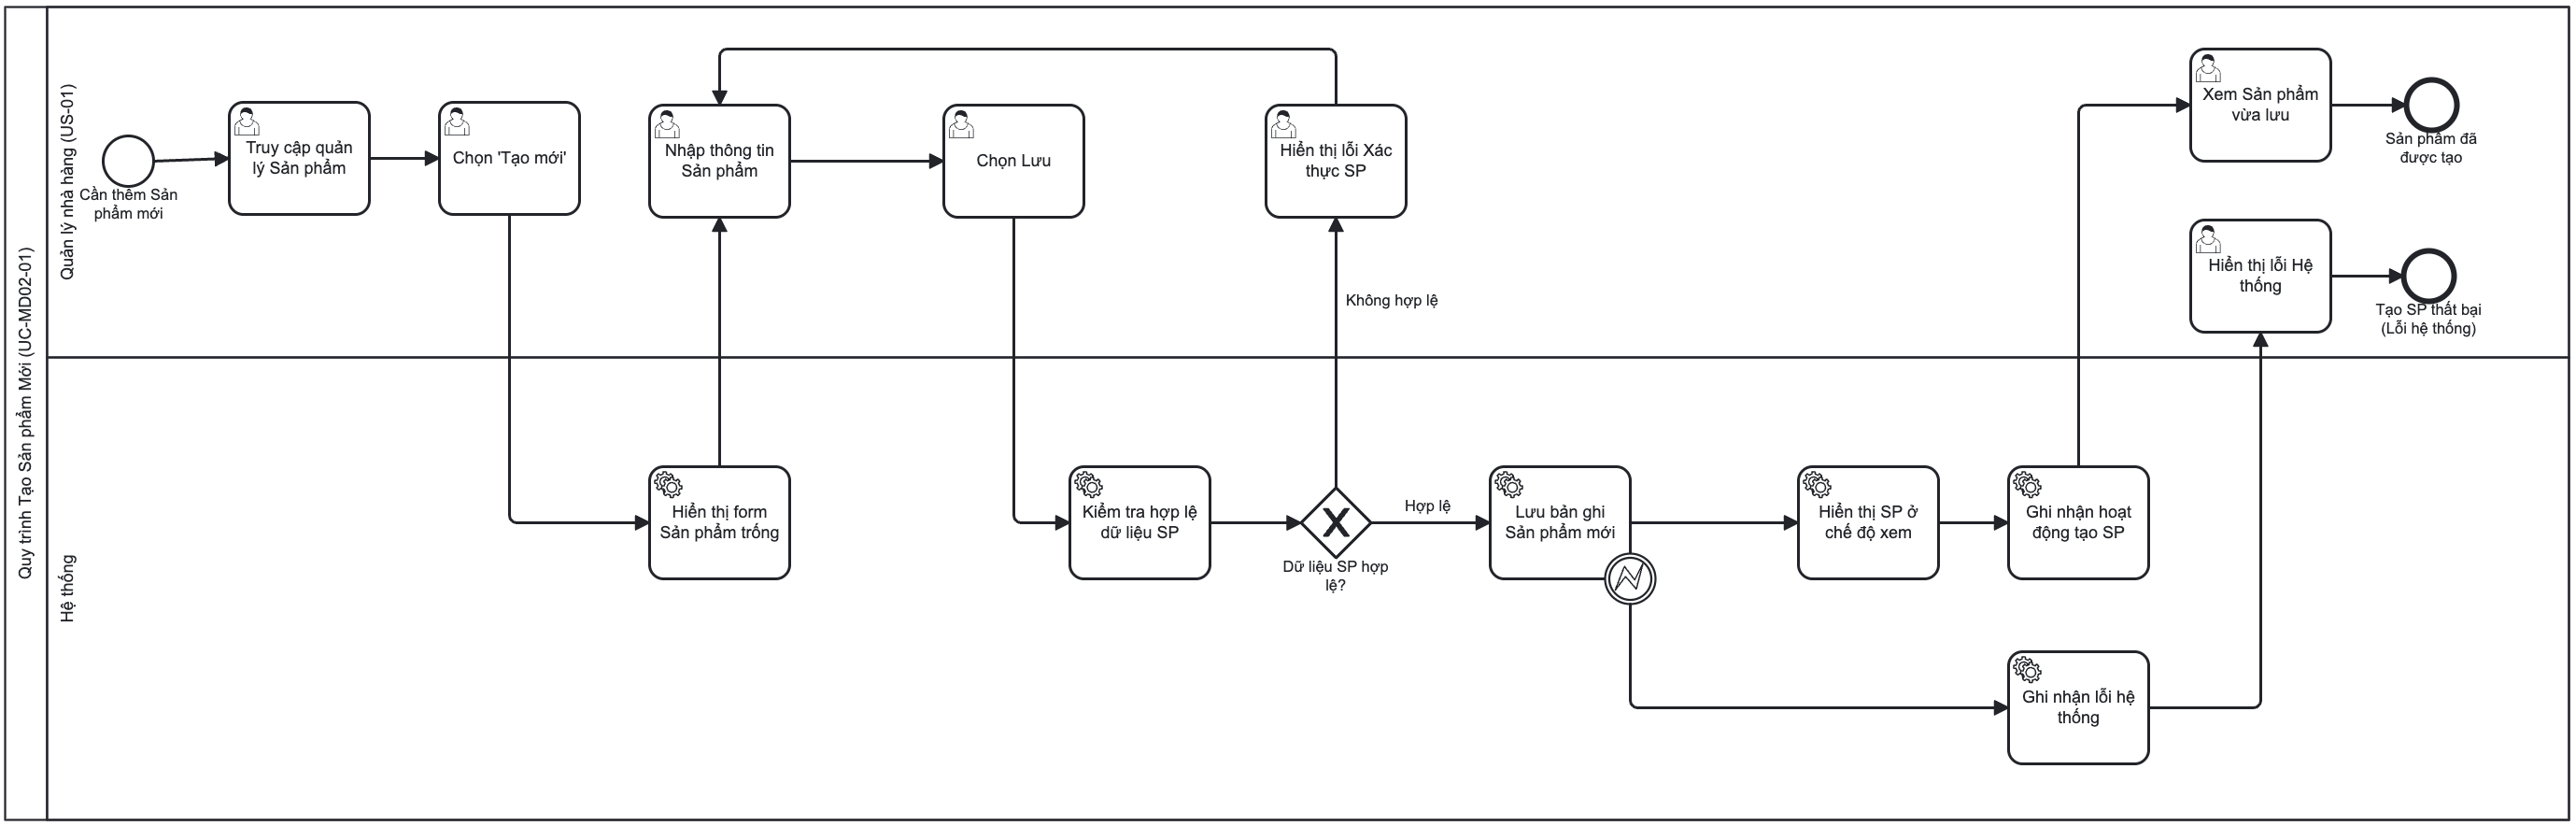
\includegraphics[width=15cm]{Sections/tong_quan/functional_spec/img/2.1.png}

     \vspace{0.5cm}
    \caption{Quy trình Tạo ca làm việc mới (UC-MD-1-01)}
\end{figure}

\subsubsubsection{FR-MD01-01: Tạo ca làm việc mới}

\begin{figure}[H]
	\centering
	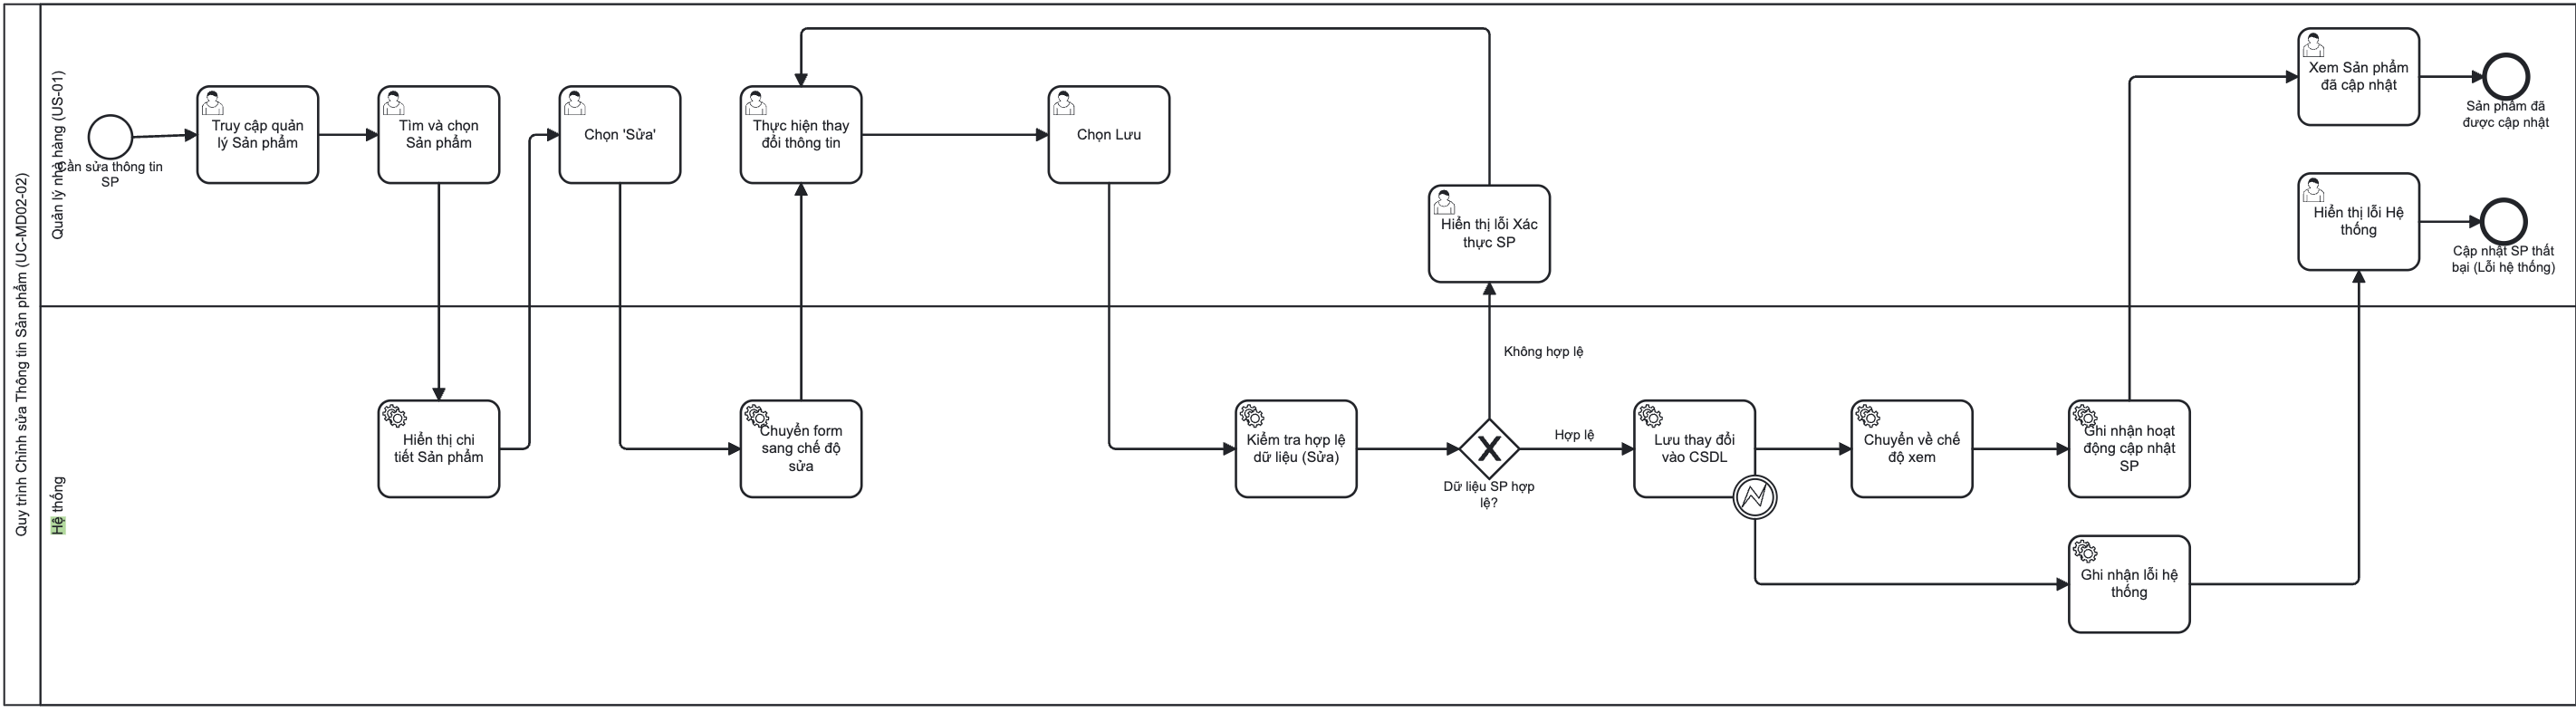
\includegraphics[width=15cm]{Sections/tong_quan/functional_spec/img/2.2.png}

     \vspace{0.5cm}
    \caption{Quy trình Tạo ca làm việc mới (UC-MD-1-01)}
\end{figure}
\subsubsubsection{FR-MD01-01: Tạo ca làm việc mới}

\begin{figure}[H]
	\centering
	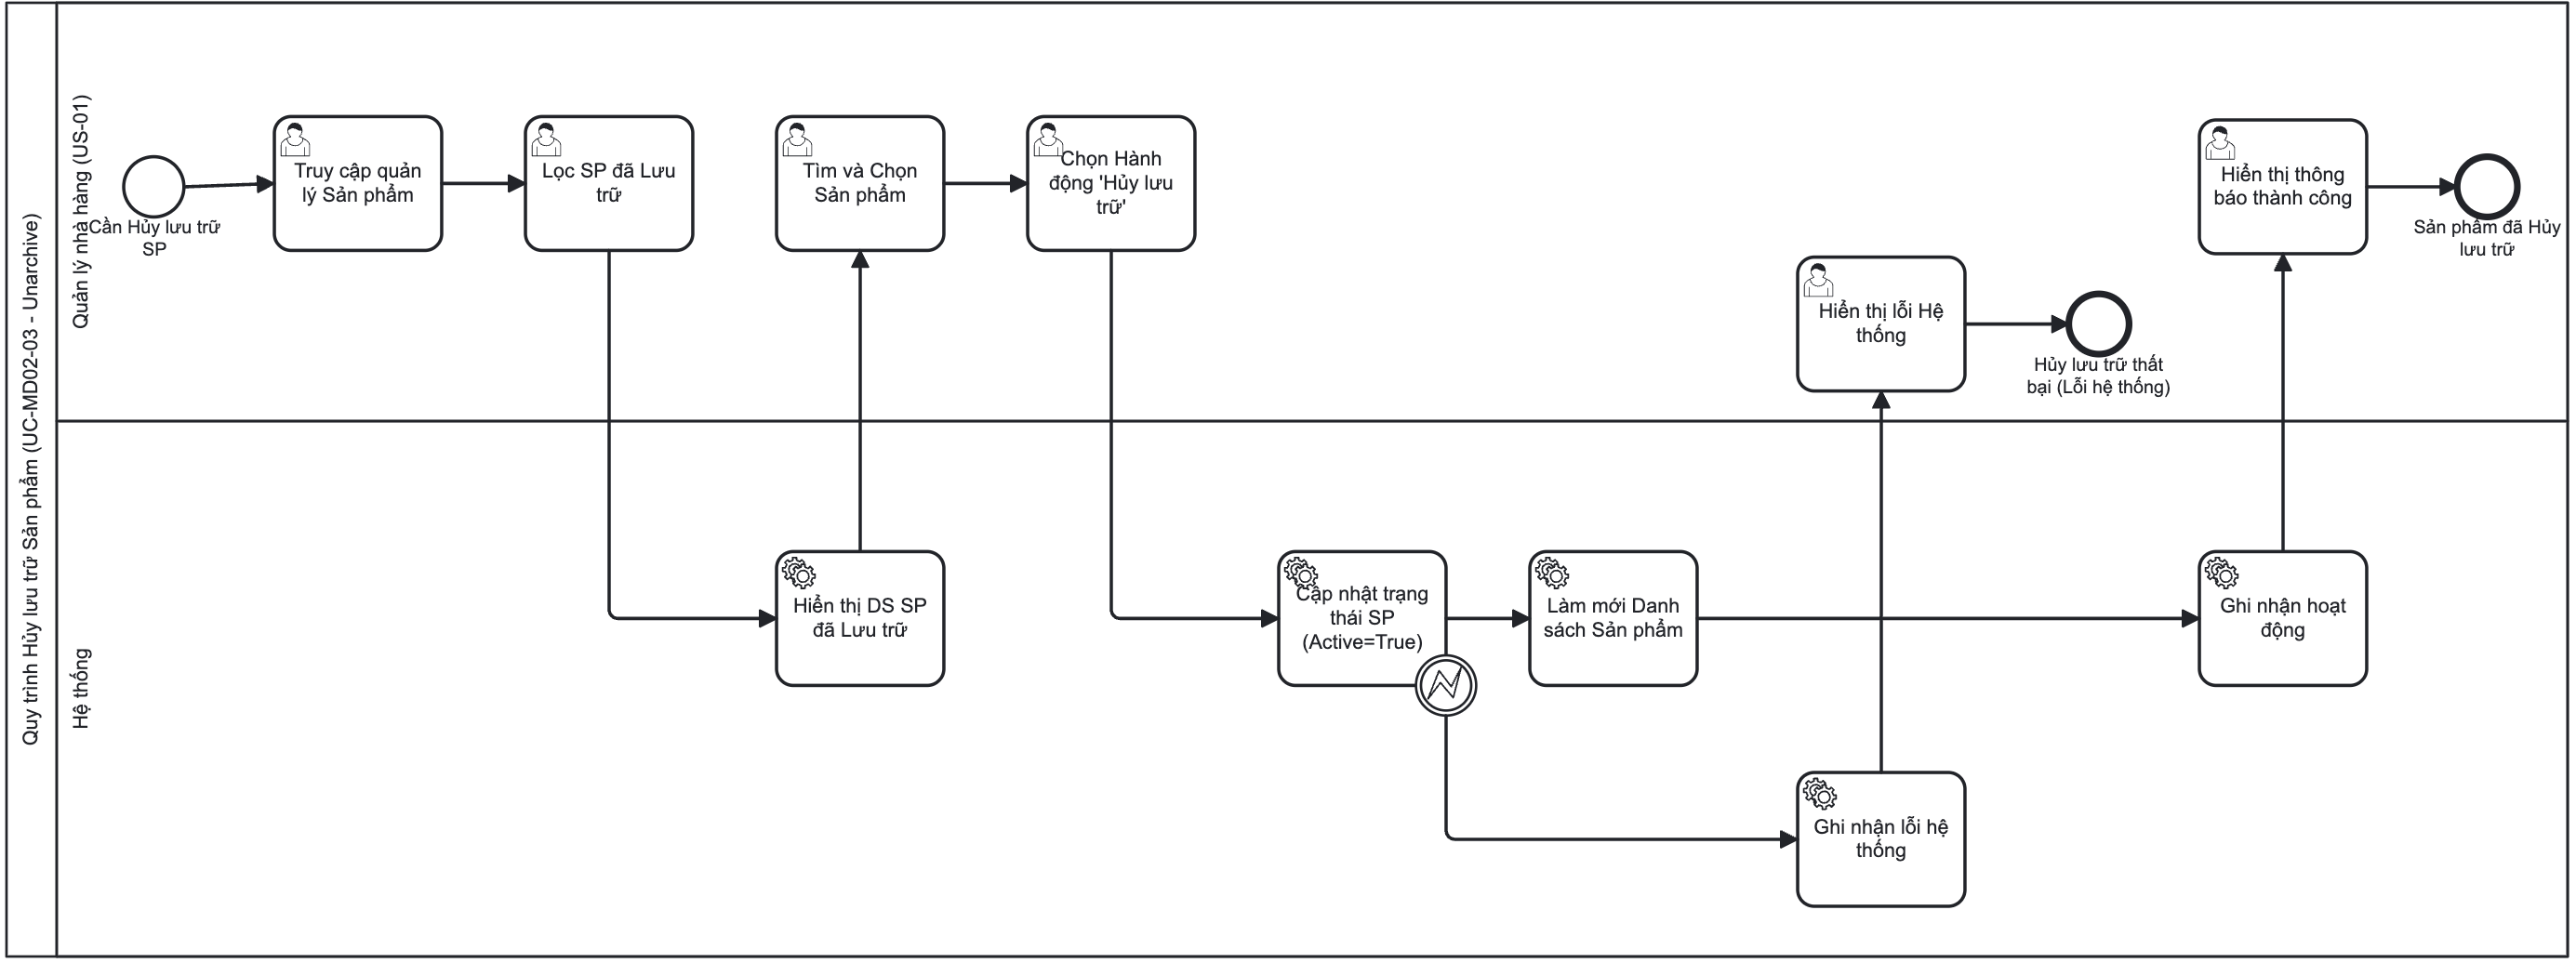
\includegraphics[width=15cm]{Sections/tong_quan/functional_spec/img/2.3.1.png}

     \vspace{0.5cm}
    \caption{Quy trình Tạo ca làm việc mới (UC-MD-1-01)}
\end{figure}

\begin{figure}[H]
	\centering
	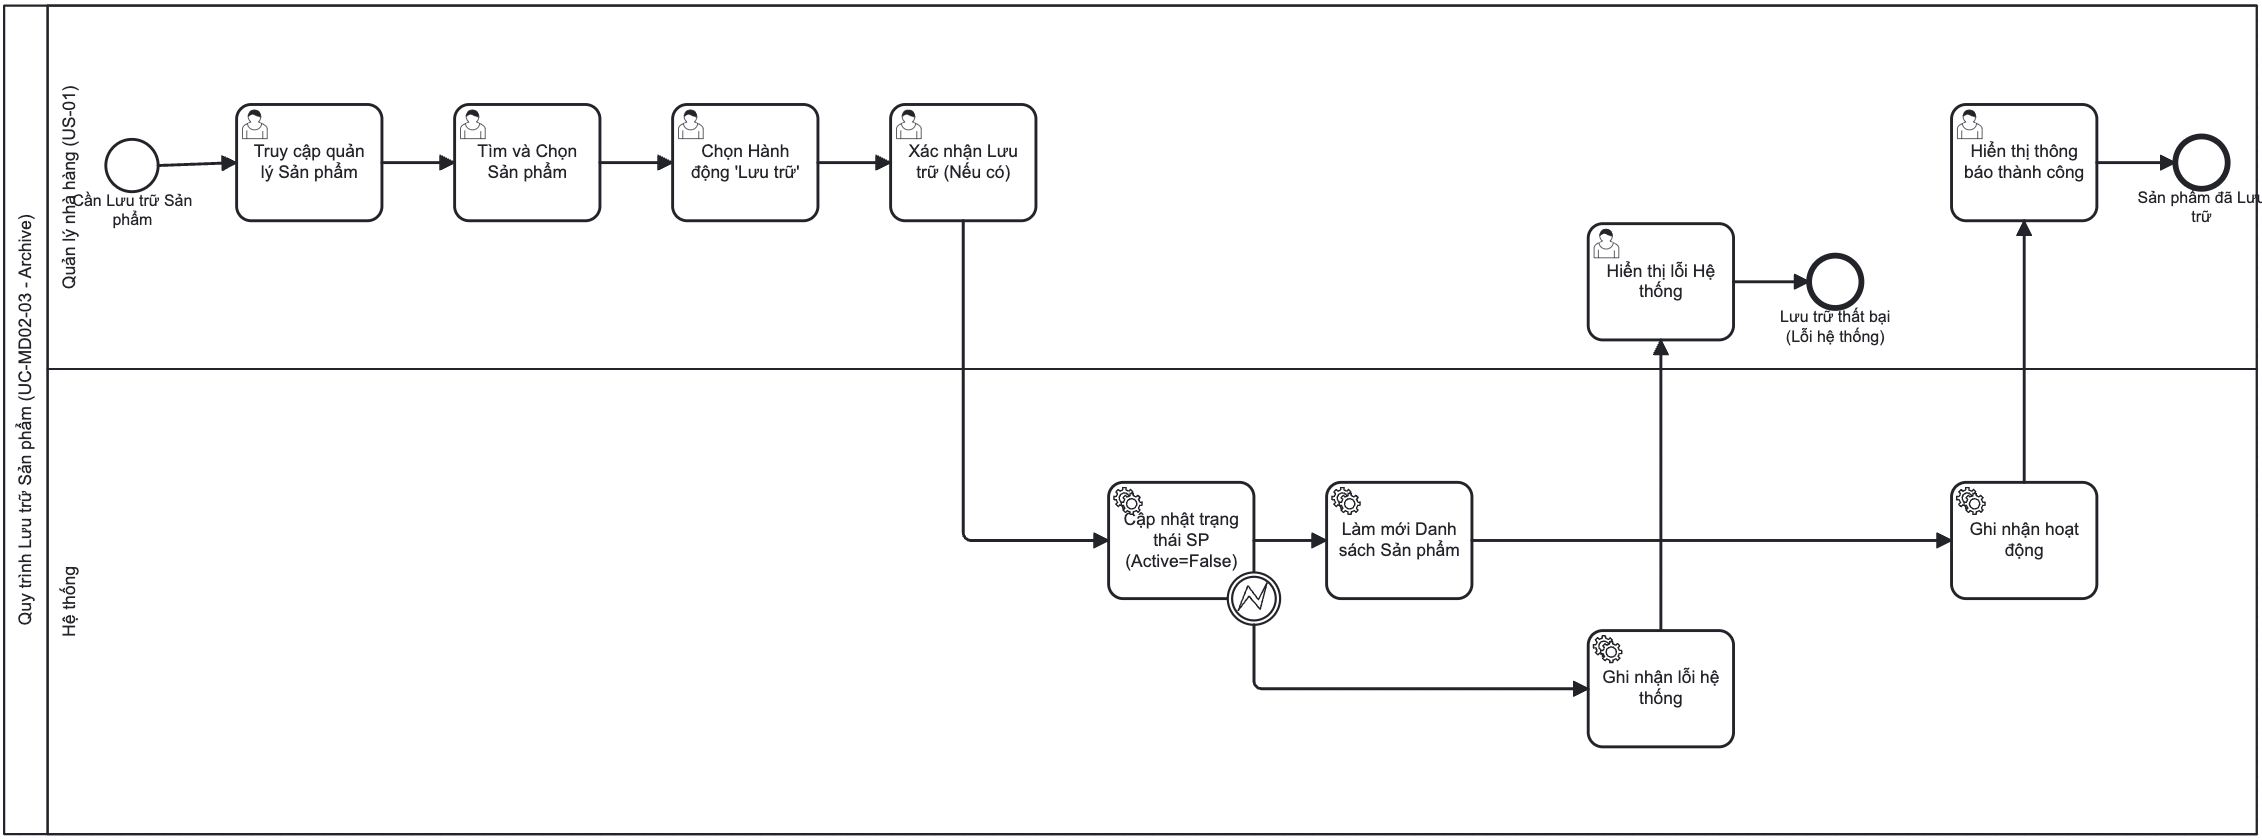
\includegraphics[width=15cm]{Sections/tong_quan/functional_spec/img/2.3.2.png}

     \vspace{0.5cm}
    \caption{Quy trình Tạo ca làm việc mới (UC-MD-1-01)}
\end{figure}
\subsubsubsection{FR-MD01-01: Tạo ca làm việc mới}

\begin{figure}[H]
	\centering
	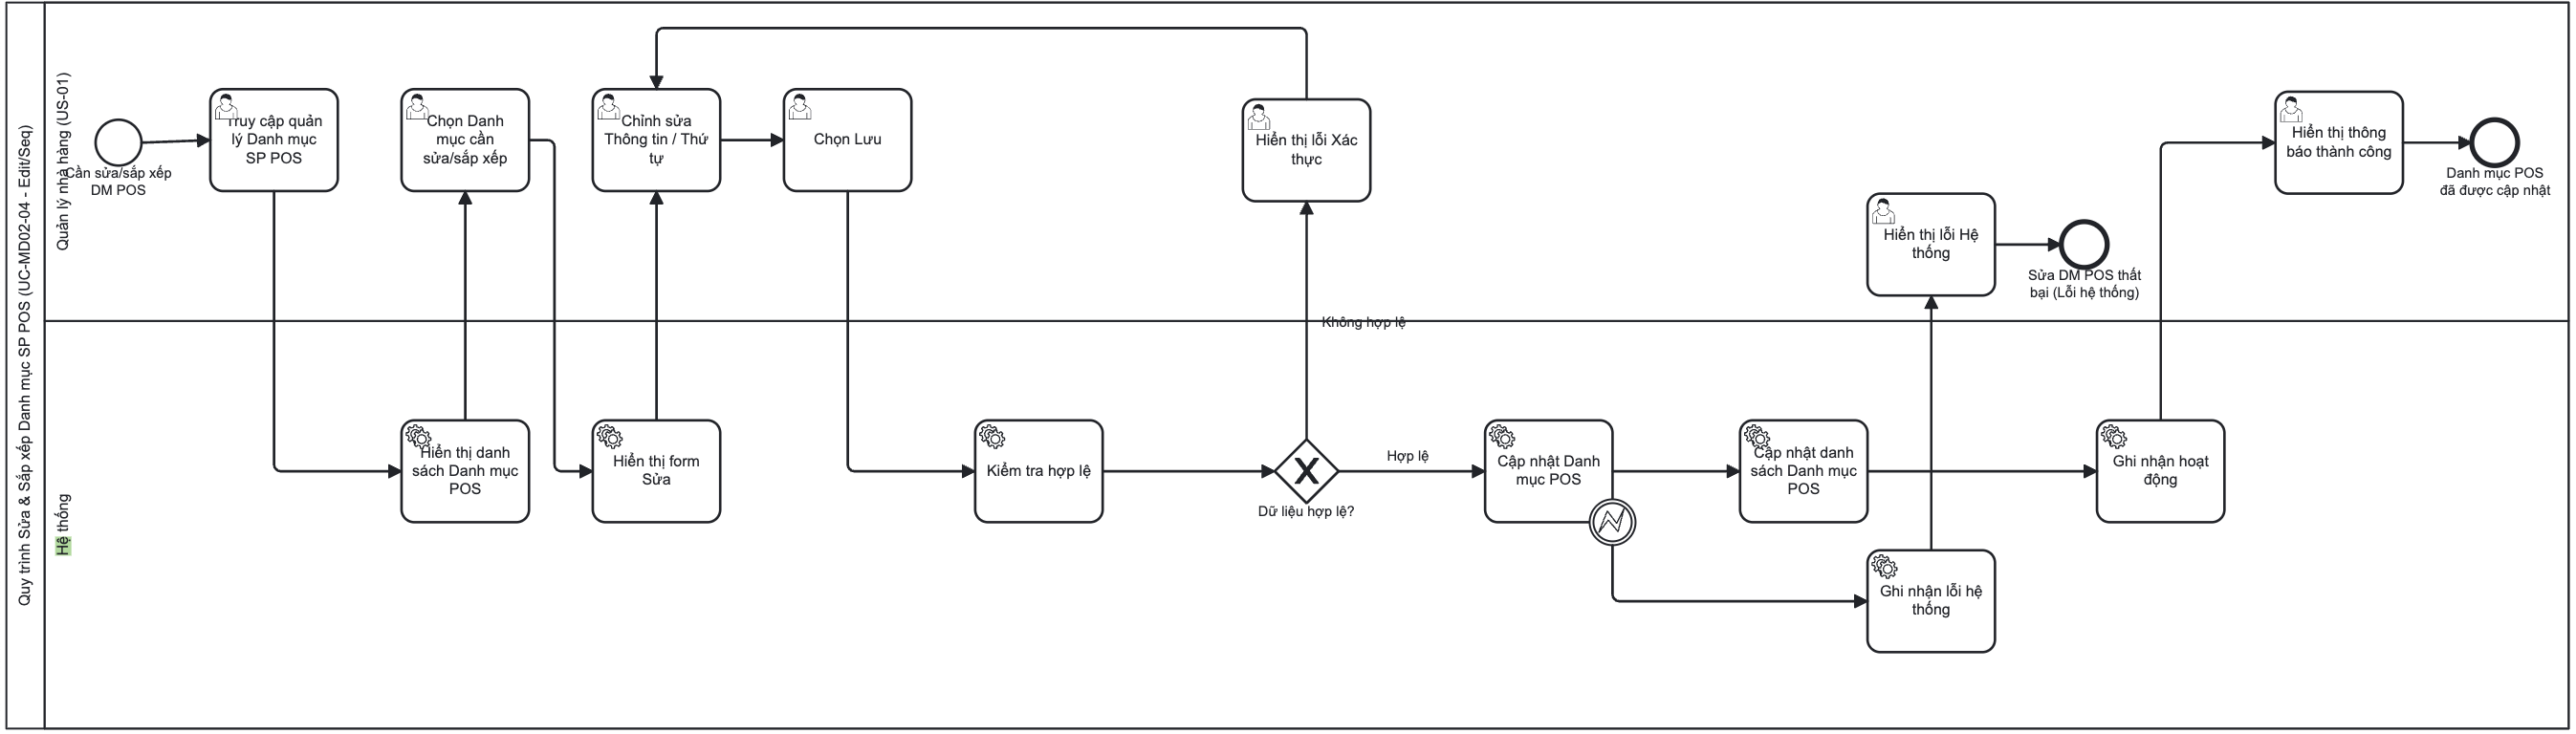
\includegraphics[width=15cm]{Sections/tong_quan/functional_spec/img/2.4.1.png}

     \vspace{0.5cm}
    \caption{Quy trình Tạo ca làm việc mới (UC-MD-1-01)}
\end{figure}

\begin{figure}[H]
	\centering
	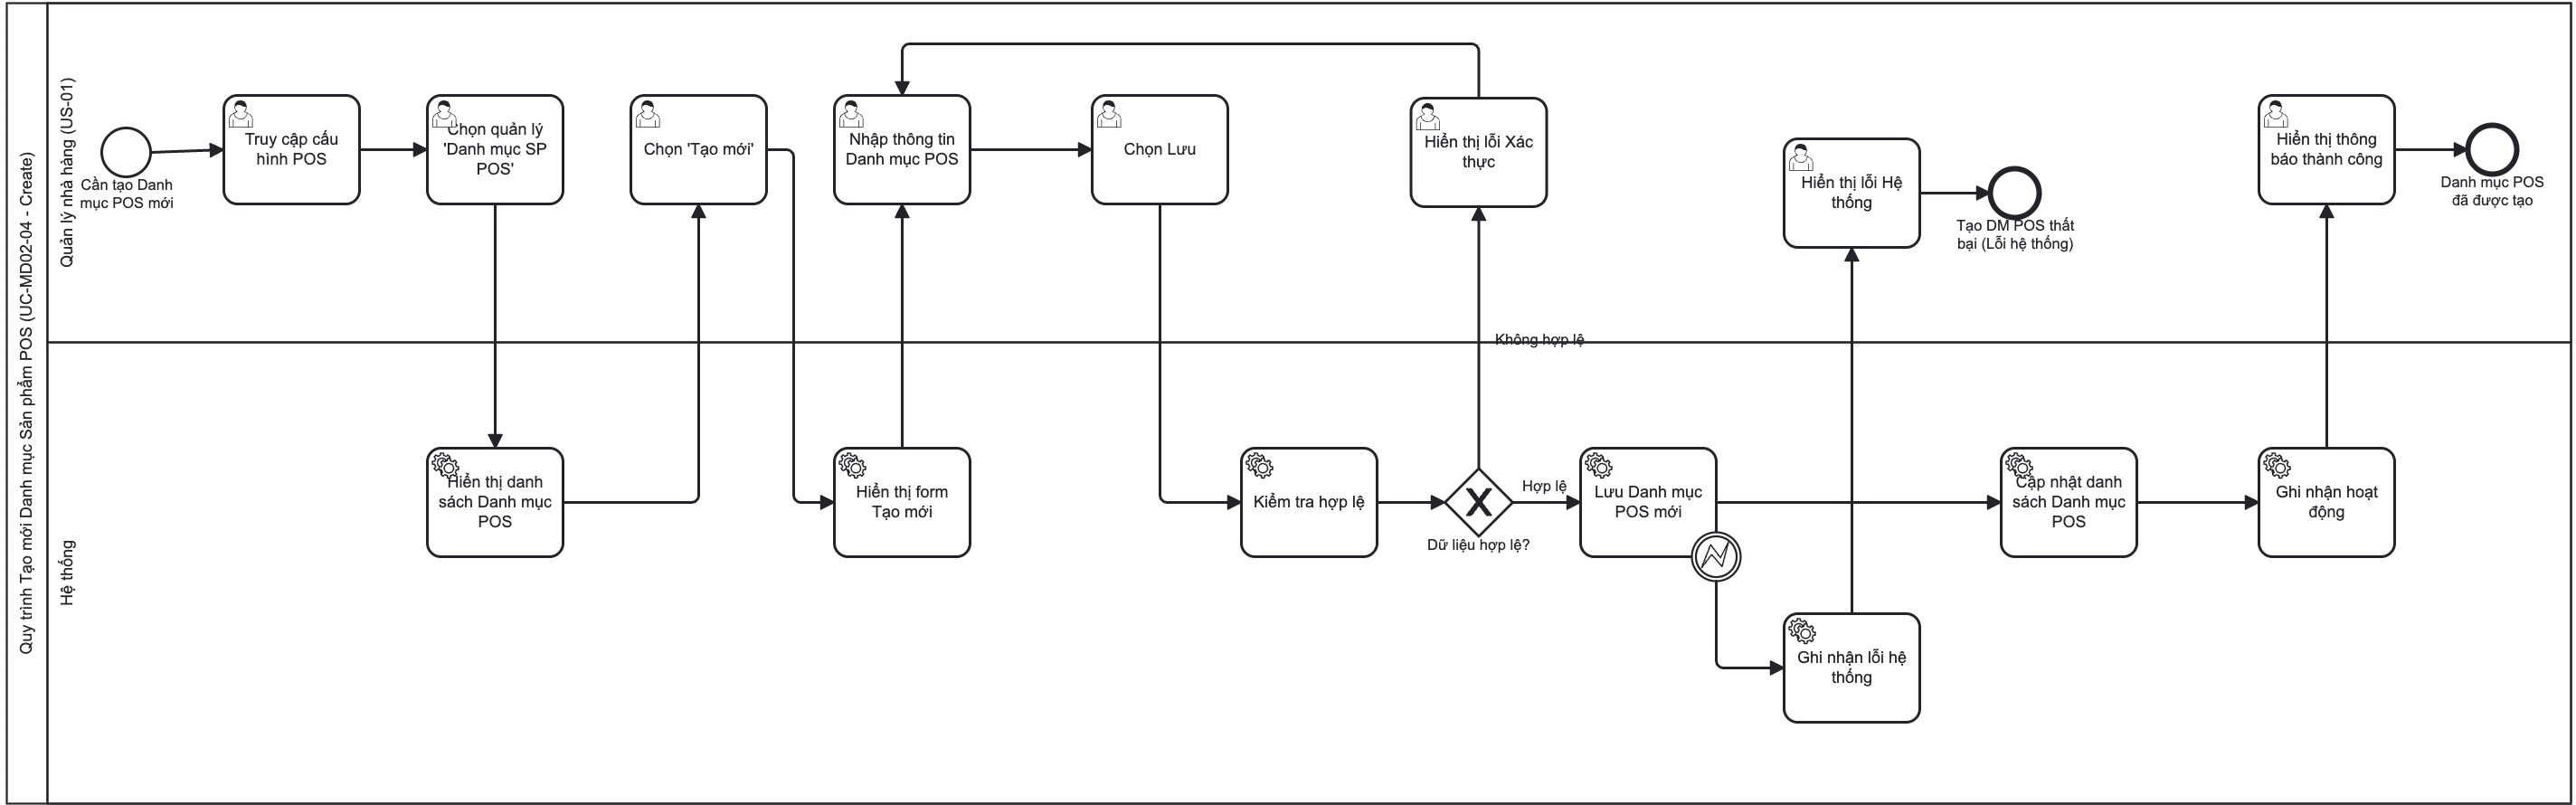
\includegraphics[width=15cm]{Sections/tong_quan/functional_spec/img/2.4.png}

     \vspace{0.5cm}
    \caption{Quy trình Tạo ca làm việc mới (UC-MD-1-01)}
\end{figure}
\subsubsubsection{FR-MD01-01: Tạo ca làm việc mới}

\begin{figure}[H]
	\centering
	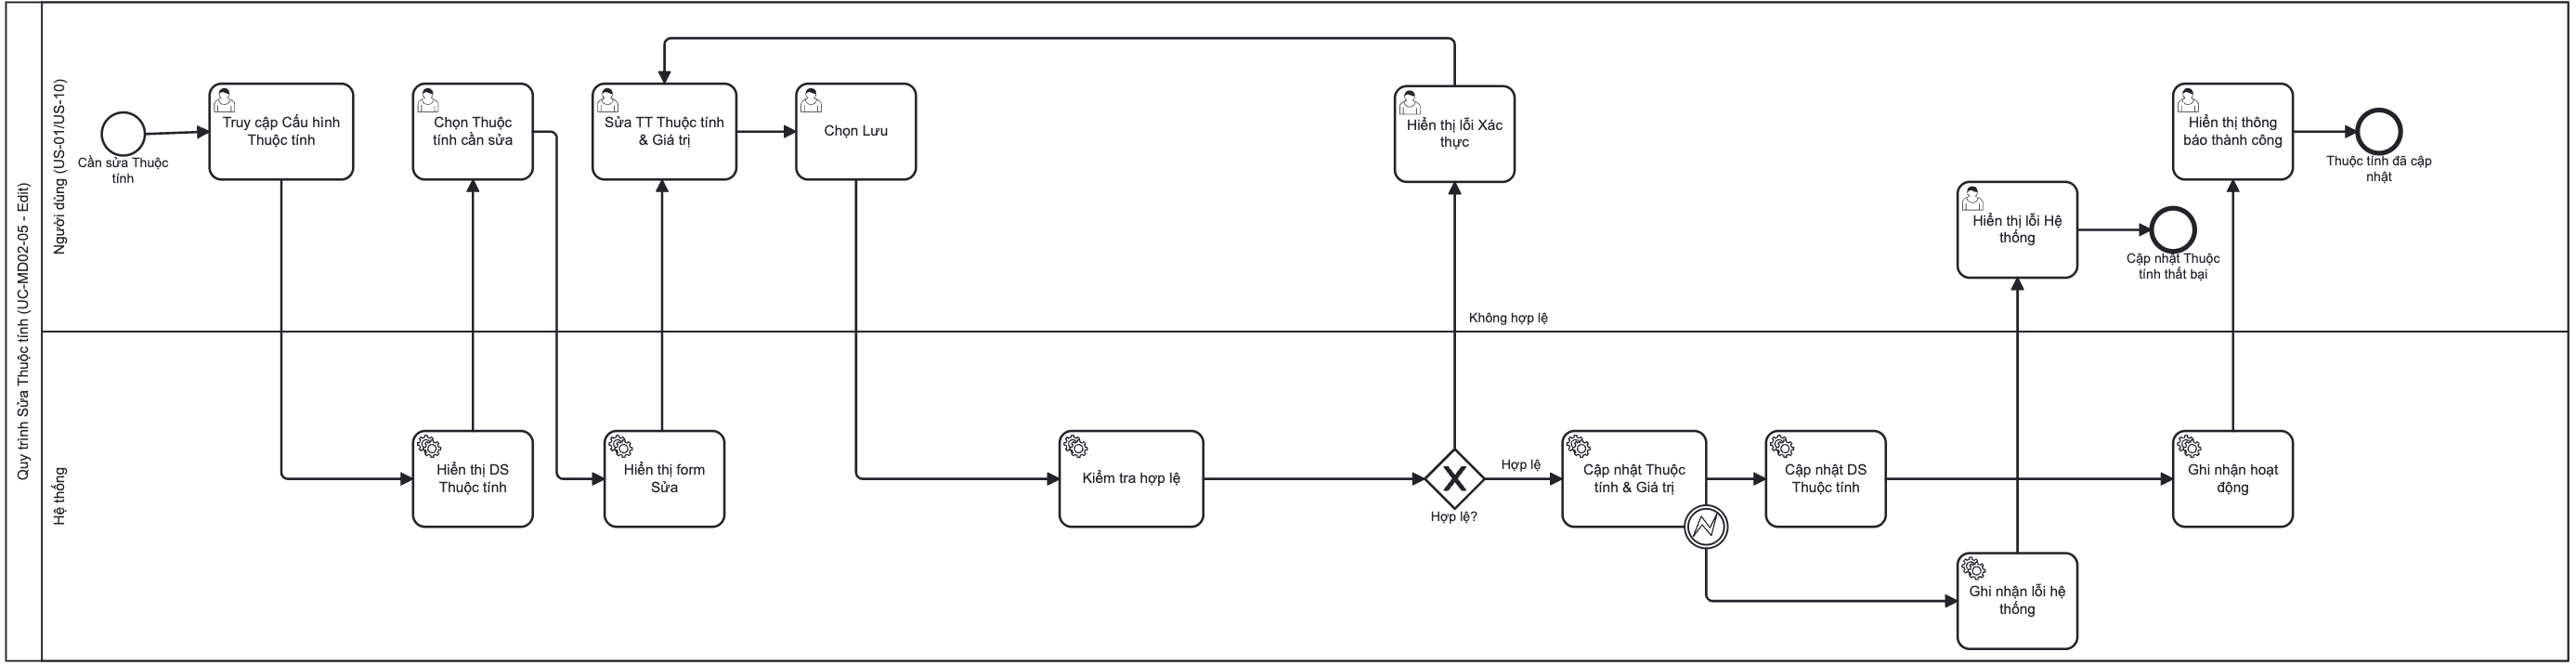
\includegraphics[width=15cm]{Sections/tong_quan/functional_spec/img/2.5.png}

     \vspace{0.5cm}
    \caption{Quy trình Tạo ca làm việc mới (UC-MD-1-01)}
\end{figure}
\begin{figure}[H]
	\centering
	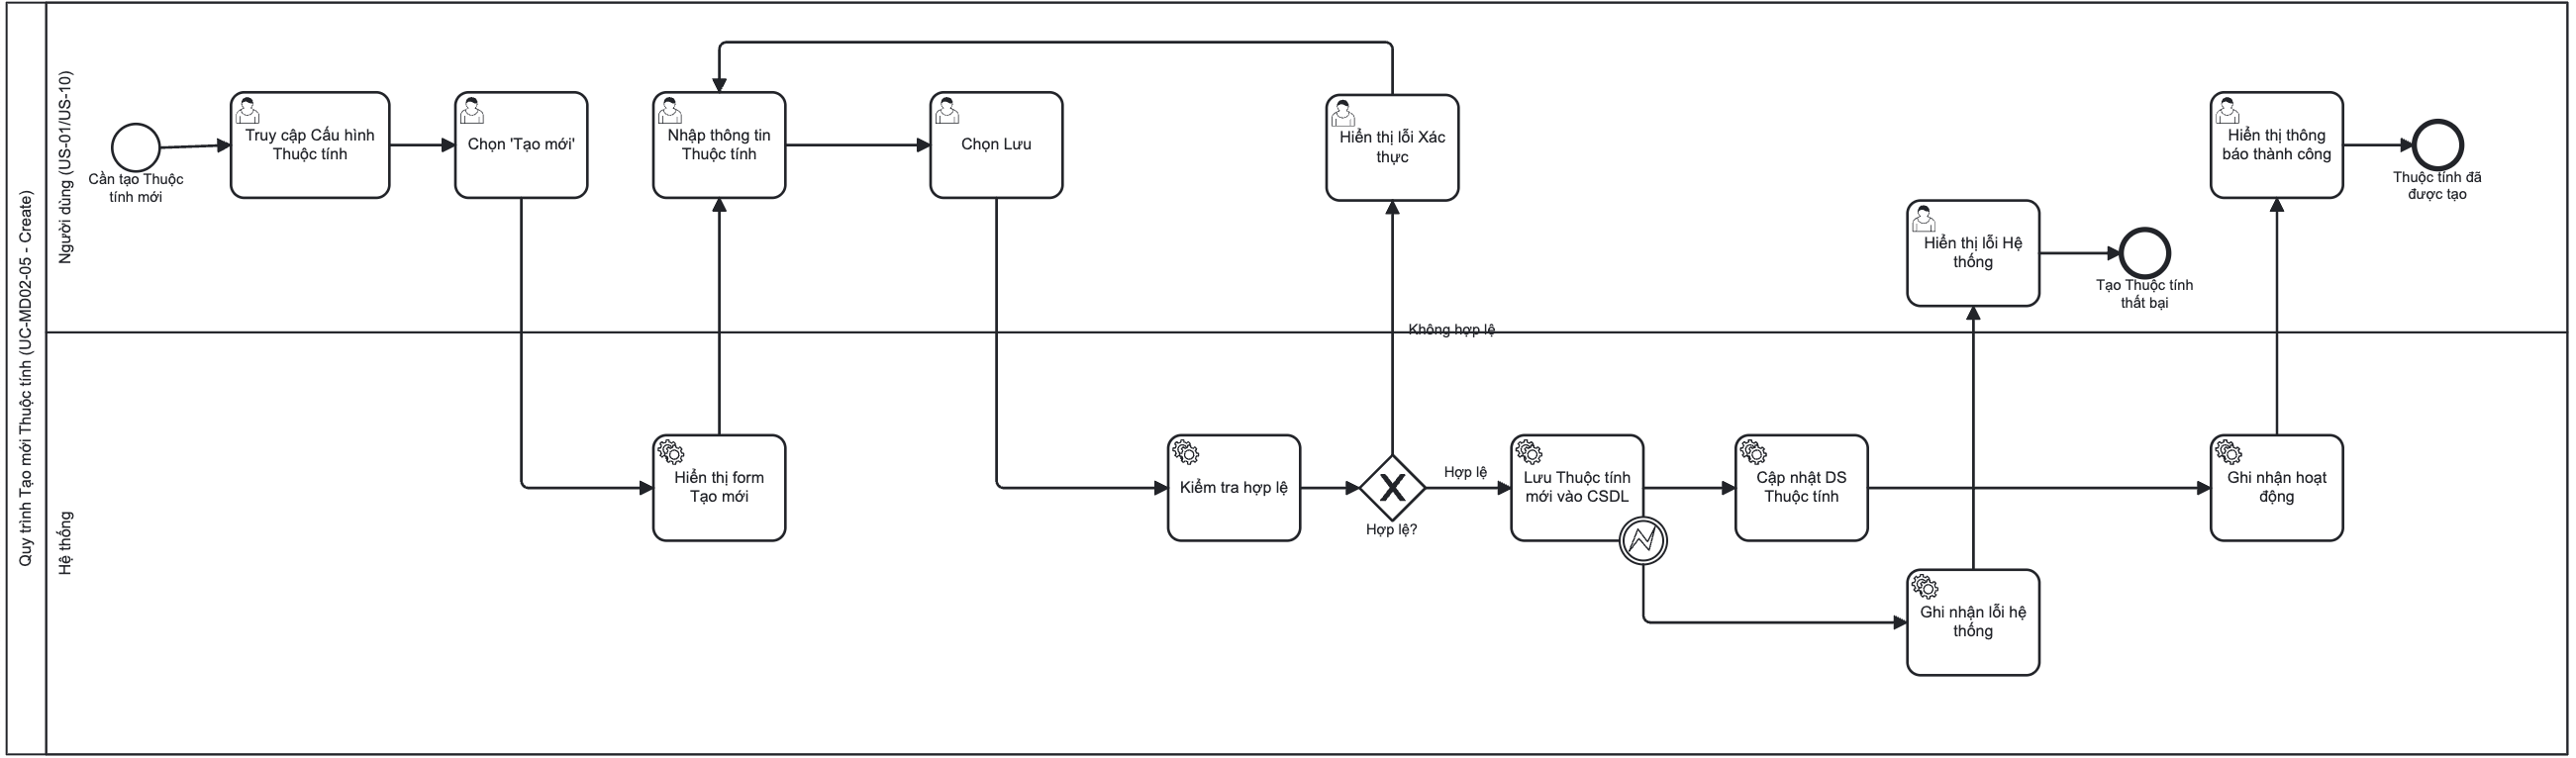
\includegraphics[width=15cm]{Sections/tong_quan/functional_spec/img/2.5.1.png}

     \vspace{0.5cm}
    \caption{Quy trình Tạo ca làm việc mới (UC-MD-1-01)}
\end{figure}
\begin{figure}[H]
	\centering
	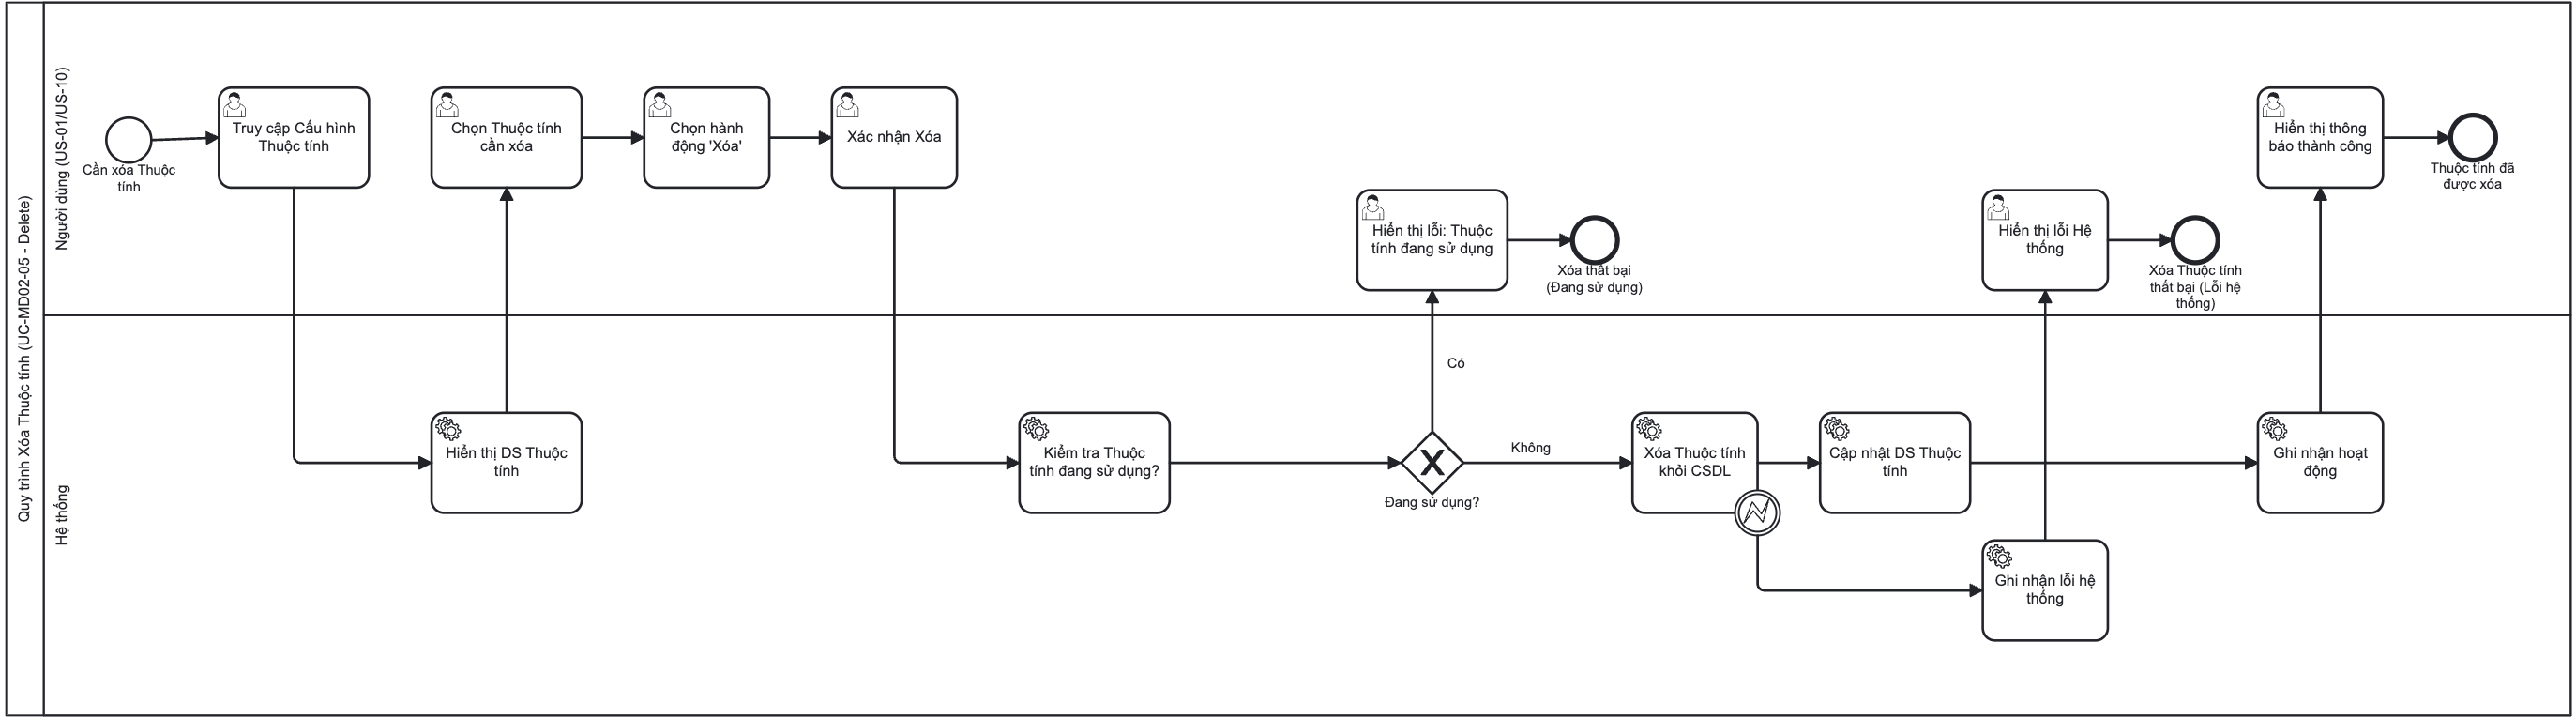
\includegraphics[width=15cm]{Sections/tong_quan/functional_spec/img/2.5.2.png}

     \vspace{0.5cm}
    \caption{Quy trình Tạo ca làm việc mới (UC-MD-1-01)}
\end{figure}
\subsubsubsection{FR-MD01-01: Tạo ca làm việc mới}

\begin{figure}[H]
	\centering
	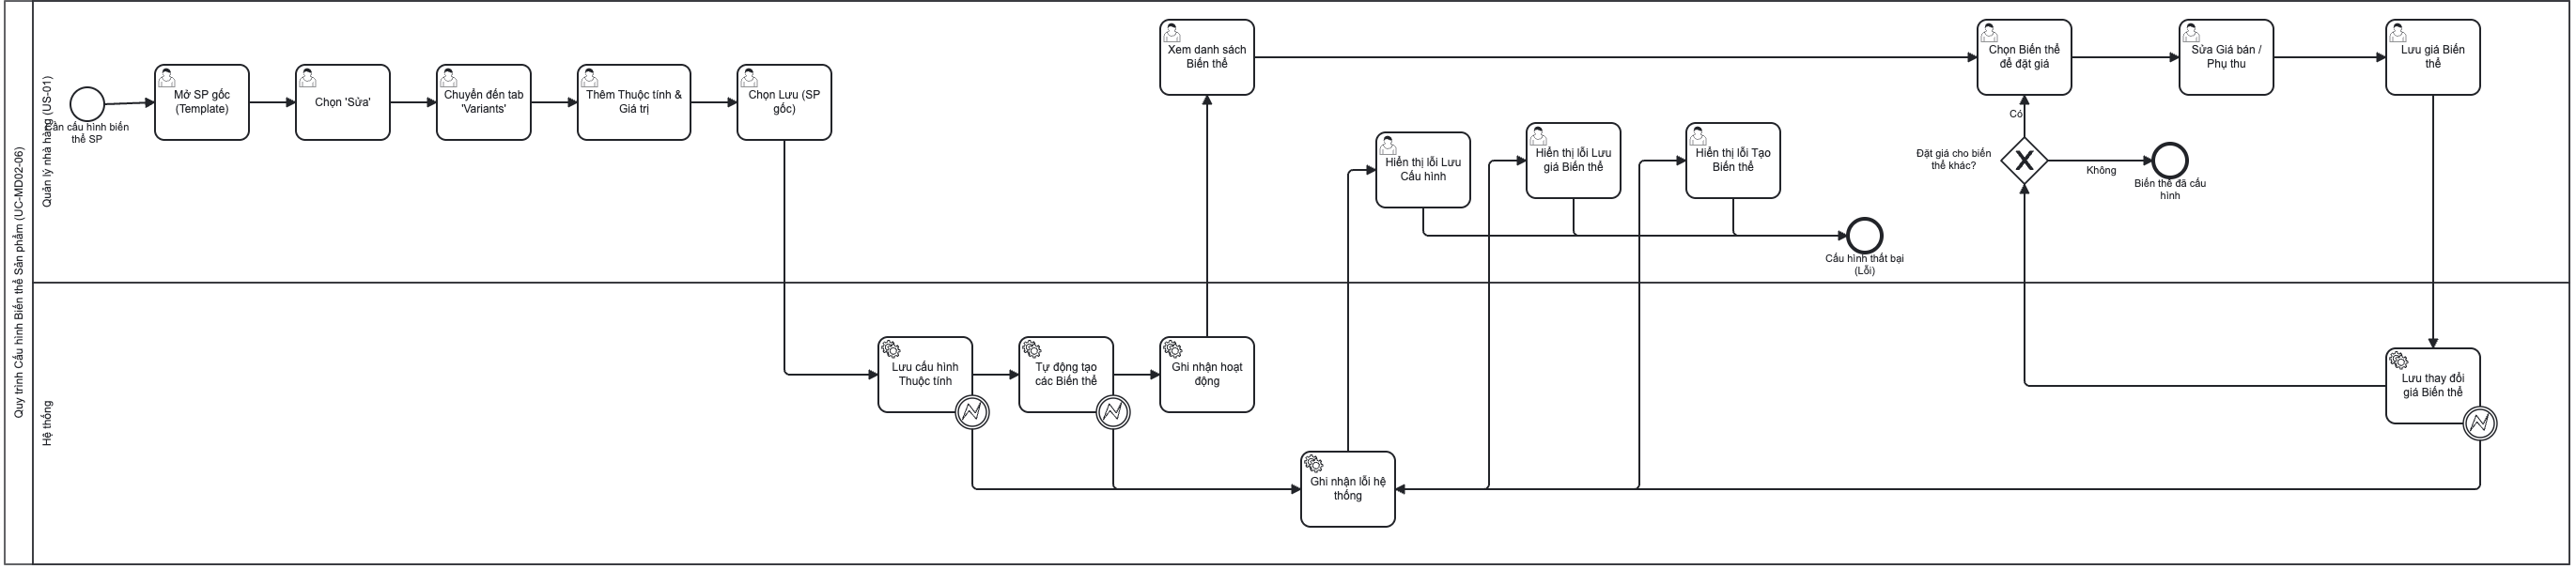
\includegraphics[width=15cm]{Sections/tong_quan/functional_spec/img/2.6.png}

     \vspace{0.5cm}
    \caption{Quy trình Tạo ca làm việc mới (UC-MD-1-01)}
\end{figure}
\subsubsubsection{FR-MD01-01: Tạo ca làm việc mới}


\subsubsubsection{FR-MD01-01: Tạo ca làm việc mới}

\begin{figure}[H]
	\centering
	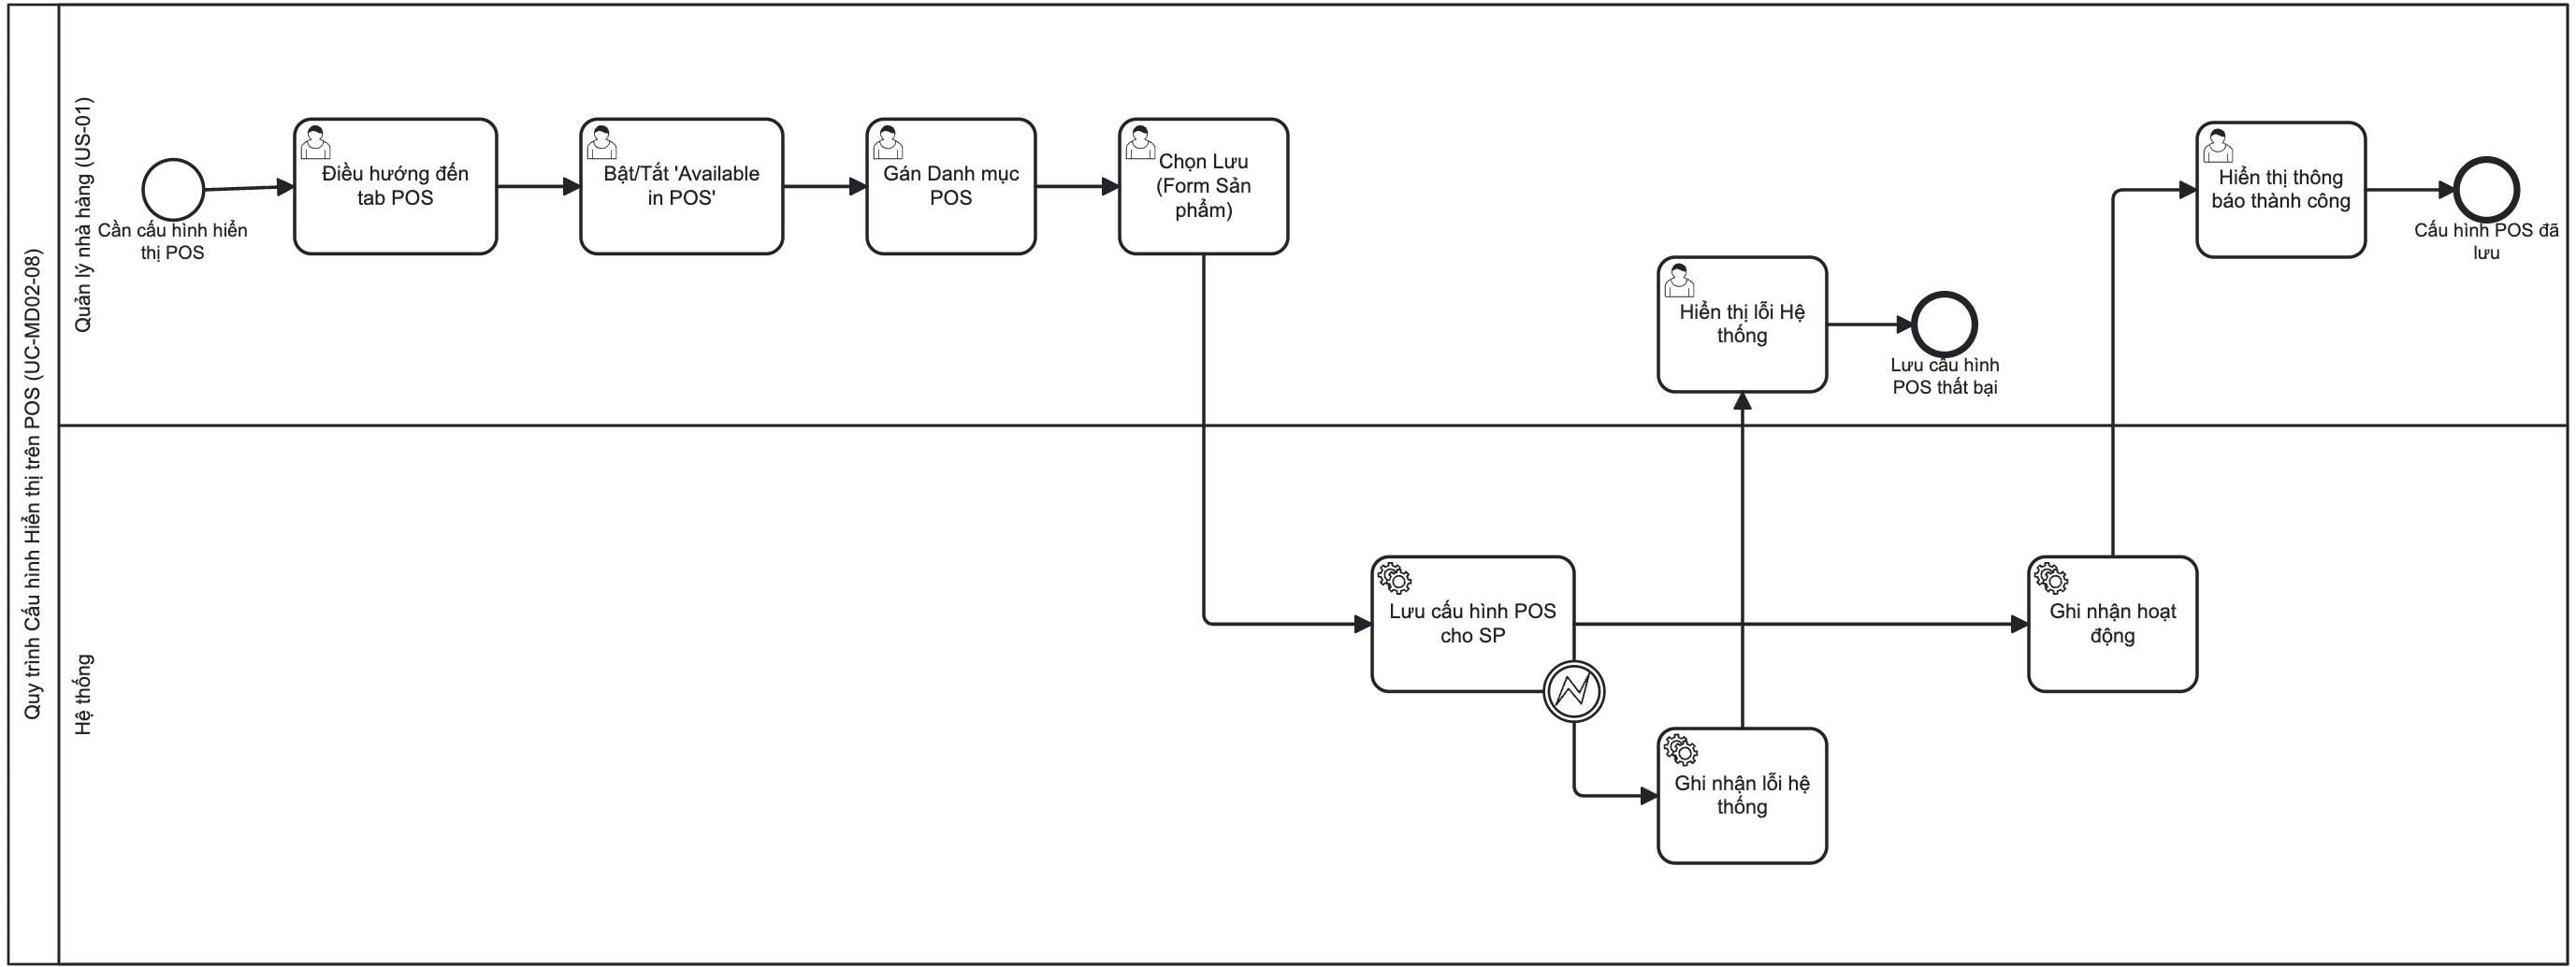
\includegraphics[width=15cm]{Sections/tong_quan/functional_spec/img/2.8.png}

     \vspace{0.5cm}
    \caption{Quy trình Tạo ca làm việc mới (UC-MD-1-01)}
\end{figure}
\subsubsubsection{FR-MD01-01: Tạo ca làm việc mới}

\begin{figure}[H]
	\centering
	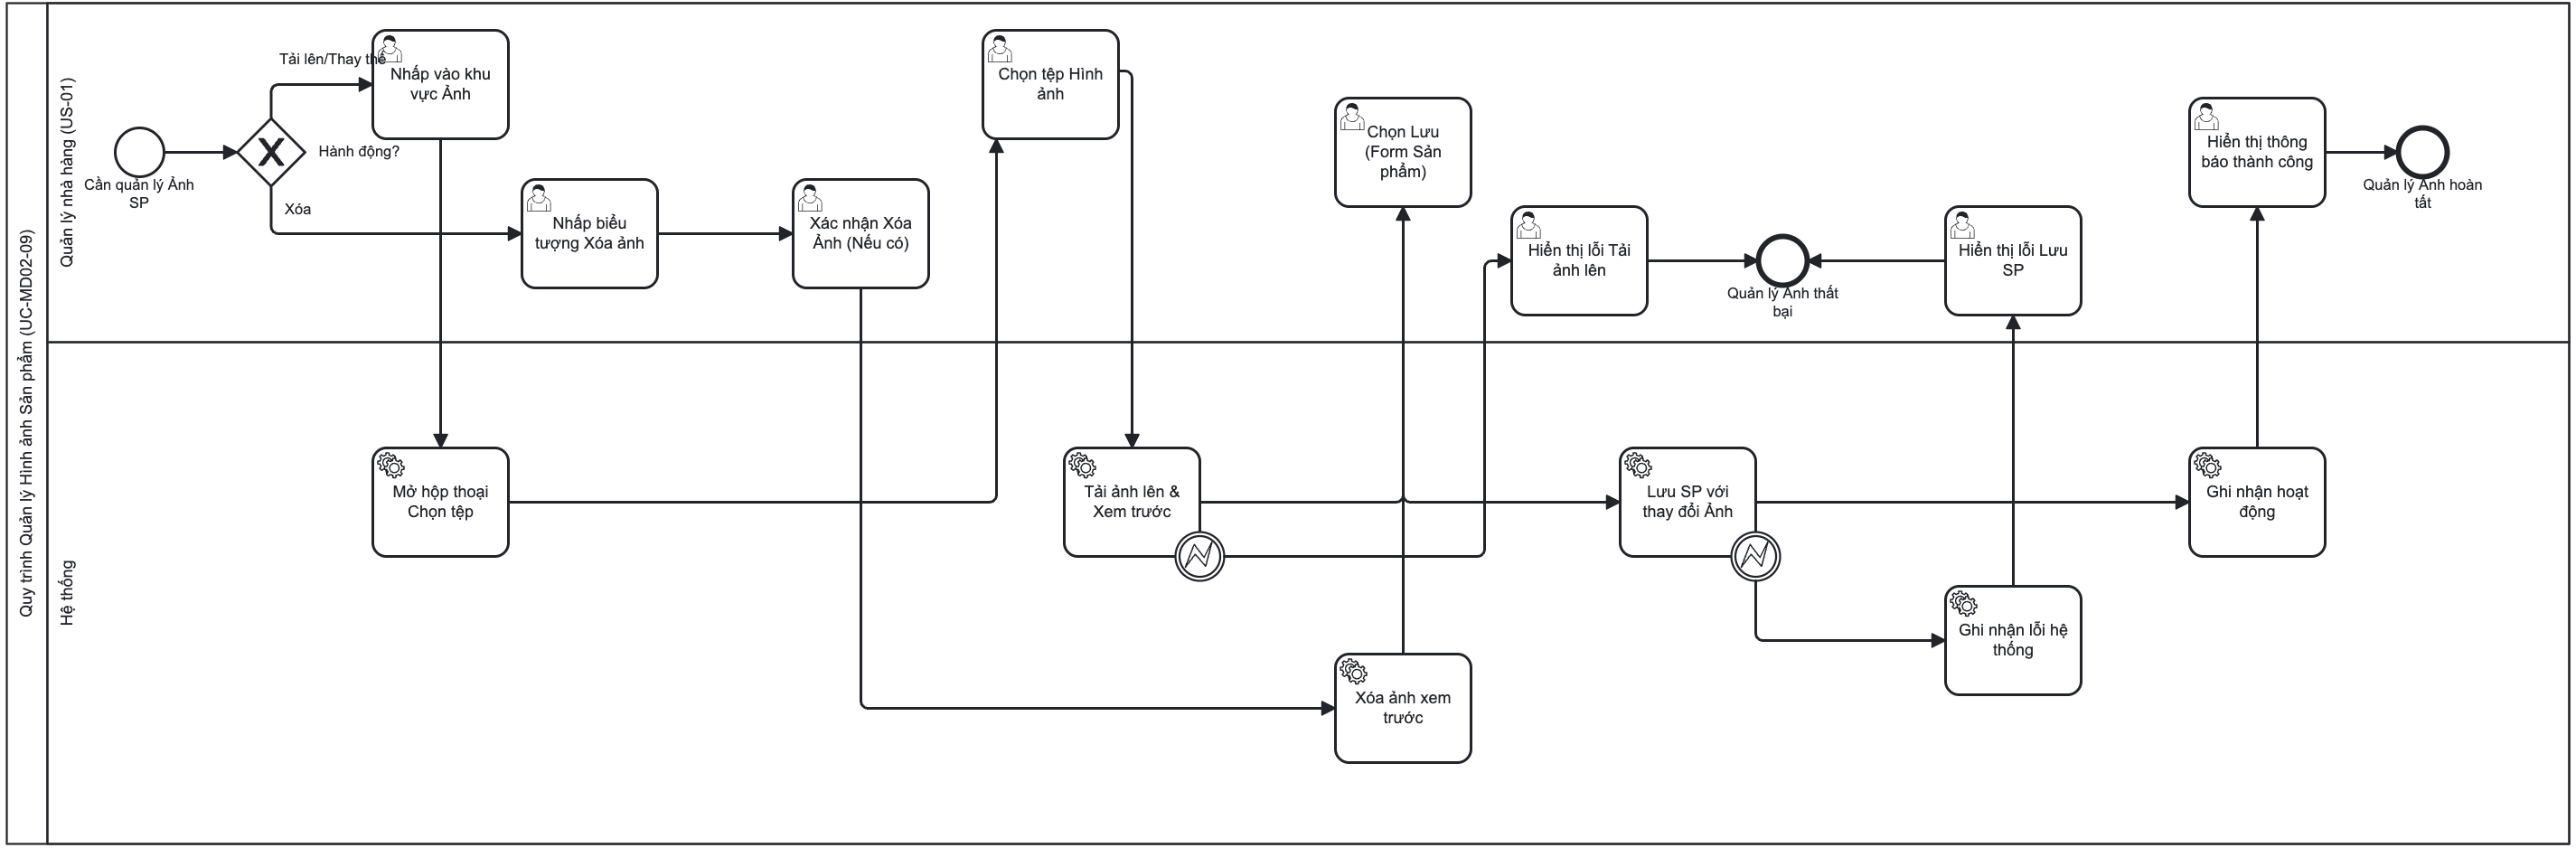
\includegraphics[width=15cm]{Sections/tong_quan/functional_spec/img/2.9.png}

     \vspace{0.5cm}
    \caption{Quy trình Tạo ca làm việc mới (UC-MD-1-01)}
\end{figure}
\subsubsubsection{FR-MD01-01: Tạo ca làm việc mới}

\begin{figure}[H]
	\centering
	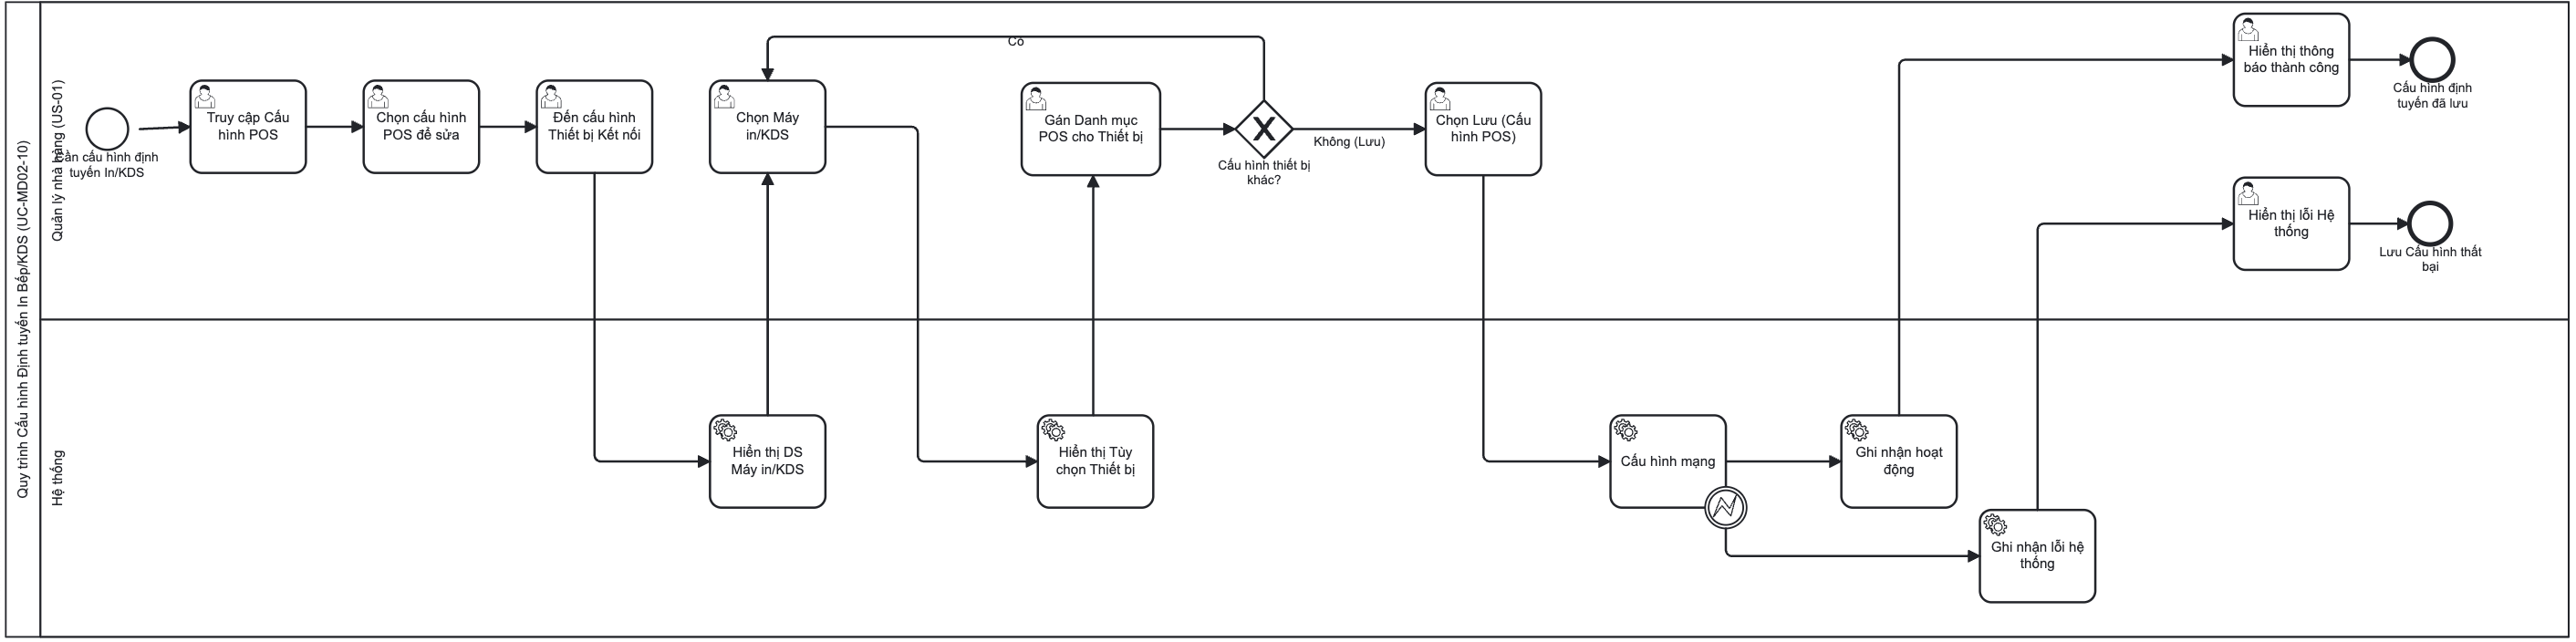
\includegraphics[width=15cm]{Sections/tong_quan/functional_spec/img/2.10.png}

     \vspace{0.5cm}
    \caption{Quy trình Tạo ca làm việc mới (UC-MD-1-01)}
\end{figure}

\subsubsubsection{FR-MD01-01: Tạo ca làm việc mới}


